\documentclass[a5paper]{article}
\usepackage[a5paper, top=8mm, bottom=8mm, left=8mm, right=8mm]{geometry}

\usepackage{polyglossia}
\setdefaultlanguage[babelshorthands=true]{russian}
\usepackage{minted}

\usepackage{fontspec}
\setmainfont{FreeSerif}
\newfontfamily{\russianfonttt}[Scale=0.7]{DejaVuSansMono}

\usepackage[font=scriptsize]{caption}

\usepackage{amsmath}
\usepackage{amssymb,amsfonts,textcomp}
\usepackage{color}
\usepackage{array}
\usepackage{hhline}
\usepackage{cite}
\usepackage{ulem}

\usepackage[xetex,linktocpage=true,plainpages=false,pdfpagelabels=false]{hyperref}
\hypersetup{colorlinks=true, linkcolor=blue, citecolor=blue, filecolor=blue, urlcolor=blue, pdftitle=1, pdfauthor=, pdfsubject=, pdfkeywords=}

\usepackage{tabu}

\usepackage{graphicx}
\usepackage{indentfirst}
\usepackage{multirow}
\usepackage{subfig}
\usepackage{footnote}
\usepackage{listings}

\sloppy
\pagestyle{plain}

\title{Практика 2: Пример архитектуры --- Bash}

\date{11.02.2019}

\begin{document}

\maketitle
\thispagestyle{empty}

\section{Enterprise Fizz-Buzz}

Сегодняшняя пара будет про примеры архитектур реальных приложений. Начнём мы с самого реального приложения --- FizzBuzz Enterprise Edition, созданного серьёзными бизнесменами для серьёзных бизнес-задач. Проект, естественно, сатира, высмеивающая безумные практики enterprise-программирования в Java-мире, но нам будет полезна как пример овердизайна. Мне кажется, будет проще понять, что такое хорошая архитектура, если на одном конце шкалы будет один большой класс, который всё делает, а на другой --- FizzBuzz Enterprise Edition с его подсистемой возврата перевода строки и прочими интересными архитектурными решениями. К тому же, там на самом деле используются (разумеется, не по делу) паттерны и архитектурные приёмы, которые нам пригодятся, поэтому имеет смысл рассмотреть это чудо архитектурной мысли поподробнее.

Собственно, серьёзная бизнес-задача такая:

Для чисел от 1 до 100:
\begin{itemize}
	\item если число делится на 3, вывести ``Fizz'';
	\item если число делится на 5, вывести ``Buzz'';
	\item если число делится и на 3, и на 5, вывести ``FizzBuzz'';
	\item во всех остальных случаях вывести само число.
\end{itemize}

``Правильное'' архитектурное решение можно найти тут: \url{https://github.com/EnterpriseQualityCoding/FizzBuzzEnterpriseEdition}.

\subsection{Обзор архитектуры}

Вот обзорная диаграмма, описывающая в общих чертах структуру этого проекта:

\begin{center}
	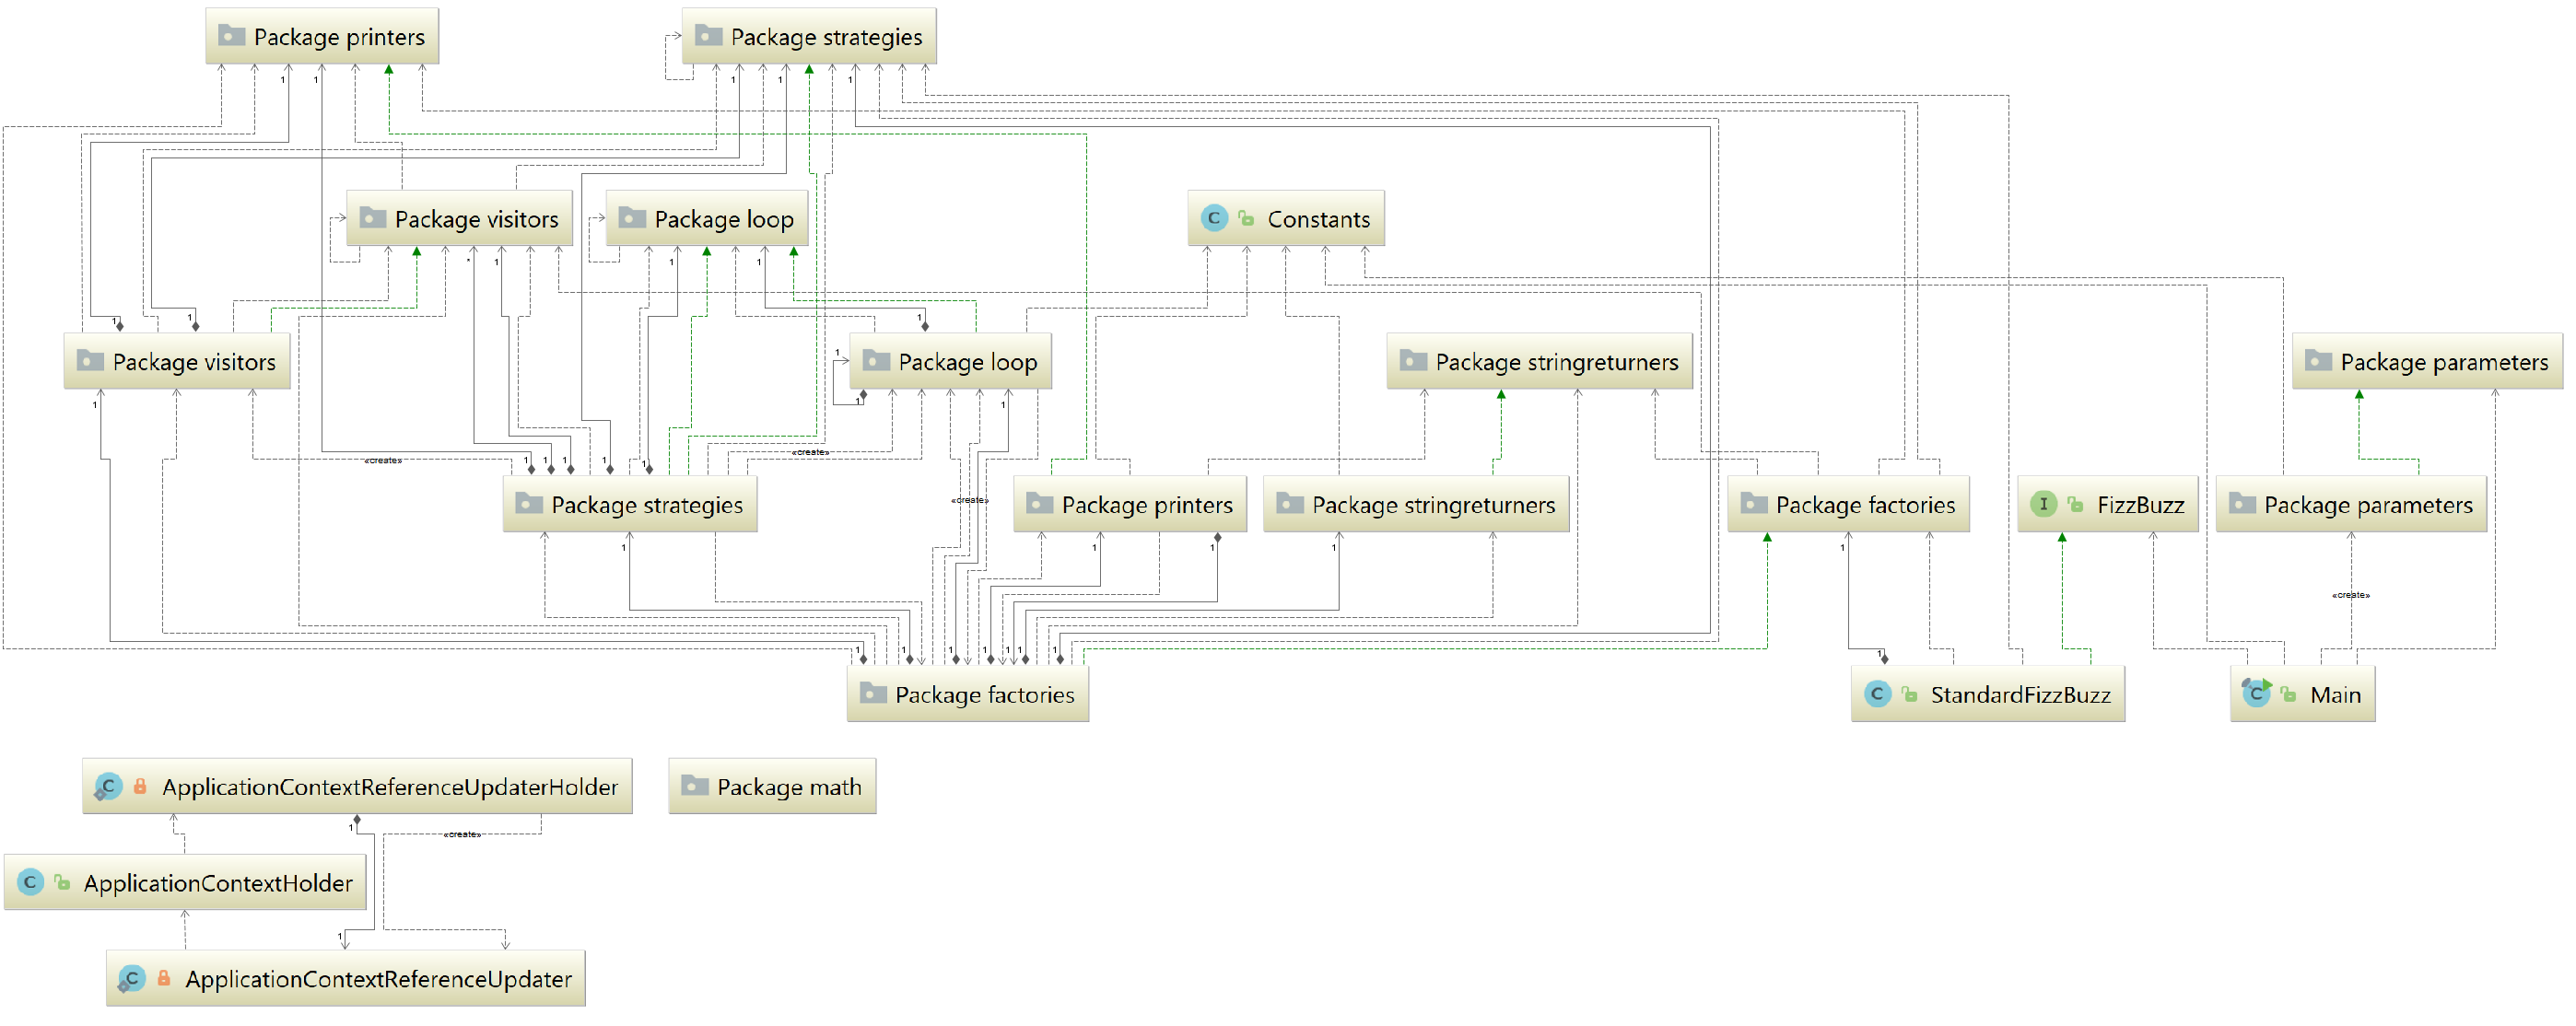
\includegraphics[width=\textwidth]{fizzBuzzArchitecture.png}
\end{center}

По данным OpenHub.net, реализация содержит 1663 содержательные строки кода и всего 40 строк комментариев (ужасно). OpenHub.net оценивает стоимость разработки этого проекта в 18К долларов.

Собственно, как всё работает: main создаёт ApplicationContext --- класс из Spring Framework, который строит систему из доступных классов, используя принцип Dependency Injection. Общая идея Dependency Injection состоит в том, что процесс создания объектов, их сборки и инициализации сложной системы --- отдельная большая подзадача, которую не стоит делать прямо в ``боевом'' коде, иначе нарушится принцип единственности ответственности. Правильнее автоматизировать этот процесс, описав набор интерфейсов, использовав эти интерфейсы в ``боевых'' классах, а затем доверив сторонней библиотеке (в нашем случае, Spring) пройтись рефлексией по нашей кодовой базе и каждому, кто в конструктор принимает объект некоторого интерфейса, автоматически подставить созданный объект класса, реализующего этот интерфейс. Звучит очень ненадёжно, но этот принцип очень активно используется в Enterprise-системах, потому что позволяет легко и приятно переконфигурировать приложения и минимизирует зависимости между классами. Дальше в курсе про Dependency Injection будет немного подробнее.

Сама логика работы реализуется классом StandardFizzBuzz, который сам решать задачу не умеет, но умеет создать стратегию решения (через фабрику стратегий, потому что он не хочет знать о конкретном классе-стратегии). Стратегия создаёт подсистему управления циклом (ну раз в условии написано про числа от 1 до 100), подсистема состоит из классов, отвечающих за границы цикла, условие завершения, и главное, действия, выполняемые на каждом шаге цикла. Ещё есть хранилище текущего контекста вычисления цикла, хранящее счётчик цикла, такие дела.

Механизм вычисления одного шага цикла тоже использует паттерн ``Стратегия'' --- сам он не хочет ничего считать, но делегирует вычисление стратегии генерации вывода. Стратегия генерации вывода принимает выходные данные, которые соответствуют счётчику цикла, но она не хочет знать про хранилище состояния цикла, в котором эти данные находятся, поэтому применяется адаптер (класс со звучным названием LoopContextStateRetrievalToSingleStepOutputGenerationAdapter), роль которого состоит в конвертации контекста цикла в параметр стратегии генерации. А вот стратегия генерации содержит в себе три стратегии вычисления, лежащие в одном списке, и для каждого значения счётчика цикла передаёт это значение всем этим трём стратегиям. Эти стратегии --- FizzStrategy, BuzzStrategy и NoFizzNoBuzzStrategy, которые про параметр цикла говорят, надо с ним что-то делать или нет (так что на самом деле это паттерн ``Спецификация'', хотя в коде он так не называется --- стратегии сами ничего не делают). Стратегии определяют, можно ли печатать Fizz, Buzz или FizzBuzz, после чего вызывается подсистема генерации, которая и печатает строку на экран.

\subsection{Чему можно научиться}

Положительные стороны этого решения такие.
\begin{itemize}
	\item Separation of Concerns --- один класс решает строго одну задачу, при этом для каждой задачи из предметной области можно указать класс, который ей занимается. Это хорошо, потому что если что-то изменится в условии, надо будет менять, скорее всего, вполне конкретный класс, результаты изменения будет легко проверить юнит-тестами (ну, по идее, в этом проекте с юнит-тестами беда). Это же способствует переиспользованию кода и вообще сопровождаемости программы ---- из маленьких кирпичиков легко собрать новую программу в той же области, чем пытаться пилить под свои задачи большие куски кода.
	\item Dependency Inversion --- реализация не должна зависеть от другой реализации, обе они должны зависеть от абстракции. В этом проекте почти никто не знает о других классах, есть чётко описанные интерфейсы, и класс может только вызывать методы по интерфейсу. Почему это хорошо --- резко снижается связность. Не важно, как реализован тот или иной интерфейс --- пока есть реализация всех нужных ему интерфейсов, наш класс будет работать. Мы можем дописывать новые реализации, изменять старые, пробовать разные реализации и даже выбирать их в зависимости от ситуации --- при этом придётся переписывать минимум кода.
	\item Dependency Injection --- становится возможным благодаря активному применению принципа Dependency Inversion. Мы можем динамически создавать и вставлять реализации интерфейсов в классы, которым эти реализации нужны. При этом используется сторонняя библиотека Spring Framework, что тоже хорошая идея --- неспецифичные для предметной области задачи, скорее всего, уже давно решены, и лучше, чем вы когда-либо сделаете.
	\item Паттерны:
	\begin{itemize}
		\item ``Фабрика'' --- для создания объектов, реализующих интерфейсы, позволяет легко менять реализацию и отделяет использование от создания;
		\item ``Стратегия'' --- инкапсулирует алгоритм работы, позволяет легко менять алгоритмы;
		\item ``Посетитель'' --- тут не особо нужен, но вообще позволяет отделить логику обхода структуры данных, состоящих из нескольких классов, от действий, выполняемых при обходе; 
		\item ``Адаптер'' --- чтобы объект, реализующий один интерфейс, мог использоваться объектом, ожидающим другой интерфейс; опять-таки, уменьшает связность системы;
		\item ``Спецификация'' --- инкапсулирует сложное логическое условие или запрос; тут используется, чтобы определиться, когда что печатать;
		\item ``Цепочка ответственности'' --- позволяет сделать список (или воообще как-то организовать цепочку) объектов, каждый из которых может обработать запрос, либо отдать дальше, если не может; тут это не совсем ``Цепочка ответственности'', потому что запрос может быть обработан двумя стратегиями сразу.
	\end{itemize}
\end{itemize}

\subsection{Почему если бы это была домашка, она была бы не зачтена}

\begin{itemize}
	\item Не выполняется принцип Keep It Simple Stupid. Хорошее решение должно быть максимально простым из тех, что всё ещё решают задачу \textbf{и} способны внятно объяснить способ её решения. Чем сложнее решение, тем сложнее его понять и, соответственно, сопровождать. Закладывать в архитектуру что-либо ``на будущее'' надо с умом, потому что, как правило, будущее так и не наступает (или наступает, но другое), а за это надо платить сложностью
	\begin{itemize}
		\item Кстати, какой-то достойный человек (жаль не помню кто) говорил ``Неправильно говорить ``строк кода написано'', правильно --- ``строк кода израсходовано'' на решение той или иной задачи''. Производительность труда программиста глупо мерять количеством строк кода, потому что из двух решений одной задачи лучше то, которое короче и проще. То есть лучше тот программист, который по традиционным метрикам работает хуже. Вообще, ниже будет ещё много слов сказано про то, что каждая строчка кода (будь то новая строка, багфикс или рефакторинг) приближает трагический конец вашей системы, потому что увеличивает её сложность и привносит дополнительный хаос. Однако это не значит, что код лучше вообще не писать, или, тем более, писать всё в одну строку, используя только однобуквенные идентификаторы --- \textit{объясняющая способность программы} важнее её размера. Программа как книга --- некоторые были бы лучше, если бы были короче (как EnterpriseFizzBuzz), некоторые были бы лучше, если бы были длиннее (как многие олимпиадные решения).
	\end{itemize}
	\item ``Синтаксическое'' разделение на пакеты, а не ``семантическое''. Есть пакет interfaces, есть пакет adapters и т.д. Мне как читателю программы такое разбиение на пакеты ничего не говорит, я и так вижу, что там, например, одни интерфейсы. А вот то, что классы, отвечающие за определение, Fizz это или Buzz, классы, отвечающие за печать, и класс, отвечающий за решение в целом, свалены в одну папку --- не очень, потому что надо вчитываться в код, чтобы понять, как они взаимосвязаны. Выше была показана структурная диаграмма проекта, там были выделены подсистемы, и эти подсистемы, хоть и выделяются по смыслу (и выделяются в потоке управления), никак не выделяются в коде. На самом деле, это индикатор более глубокой и серьёзной проблемы --- отсуствие модульности как таковой. Классы хоть и не взаимодействуют напрямую, но представляют собой единую массу, которая вместе решает задачу, а не набор блоков, каждый из которых решает свою подзадачу и понятным образом связан с другими блоками. Это проявление антипаттерна ``Big Ball of Mud'' --- система не имеет крупномасштабной структуры, вся её архитектура определяется взаимодействием между конкретными классами.
	\item Хардкод основных параметров вычисления, иногда безумный: \mintinline{java}|public static final int INTEGER_DIVIDE_ZERO_VALUE = 0;|. Если уж enterprise, всякие штуки типа верхней и нижней границ цикла правильно грузить из XMLного конфига (ну или менее enterprise, JSON).
	\item Нет юнит-тестов, есть только несколько довольно жалких интеграционных тестов. Я бы не стал рефакторить такую систему. Вообще, возможности для юнит-тестирования тут очень высоки --- чёткое разделение ответственностей позволяет писать изолированные тесты, следование принципу Dependency Inversion позволяет вовсю применять мок-объекты.
	\item Вообще нет логирования --- если система упала, то непонятно, где и почему. Для enterprise-приложений логирование обязательно (и реально может спасти если не жизнь, то карьеру-то точно).
	\item 1663 строки кода и всего 40 строк комментариев. Архитектурного описания нет вообще (а на самом деле, очень бы пригодилось). Вновь пришедшему в проект человеку надо будет прочитать практически весь код, чтобы понять, как оно работает. Проблема особенно усугубляется отсутствием модульности и крупномасштабной структуры.
\end{itemize}

\section{Архитектура bash}

Теперь перейдём к более ``настоящему'' проекту --- командному интерпретатору Bash. Это не то чтобы хороший пример хорошей объектно-ориентированной архитектуры (он был написан на C, причём ещё в те времена, когда объектно-ориентированная архитектура была не очень модна), к тому же его архитектура не очень подробно документирована. Но нам этот проект интересен, во-первых, в свете домашки, а во-вторых тем, что его часто (ну, относительно) используют в исследованиях по архитектуре как ``подопытного кролика''. Суммарно Bash имеет около 70К содержательных строк кода, к тому же ещё использует библиотеку Readline, которая, хоть и поддерживается тем же товарищем, что и Bash, и разрабатывалась в основном для Bash-а, но формально к нему не относится и не имеет кода, специфичного для Bash.

Дальнейшее изложение будет вестись по книге A. Brown, G. Wilson, The Architecture of Open Source Applications и статье J. Garcia et al., Obtaining Ground-Truth Software Architectures (рисунки ниже оттуда и из слайдов prof. N. Medvidovic). Книга, кстати, весьма годная, редакторы собрали довольно большое количество не очень больших заметок об архитектуре известных проектов с открытым исходным кодом от их авторов или maintainer-ов. С одной строны, каждый из авторов описывает архитектуру как умеет, поэтому там всё очень неформально, не очень подробно и далеко не всегда соответствует правилам, про которые мы будем рассказывать на этом курсе. С другой стороны, как редакторы справедливо отмечают во введении, архитекторы, которые проектируют здания, в ходе учёбы изучают сотни проектов зданий и критики этих проектов от профессионалов, тогда как архитекторы ПО, как правило, знакомы только с несколькими крупными системами, и то большинство из них они сами же и проектировали. Связано это с очень большой сложностью ПО и невозможностью зачастую восстановить архитектуру по программе, так что возможность посмотреть, как другие проектируют ПО, и поучиться на их ошибках или перенять их хорошие идеи может быть очень ценной.

Вот как выглядит диаграмма, характеризующая на высоком уровне архитектуру Bash (примерно то, что я хотел увидеть на доске на первой паре, наверное):

\begin{center}
	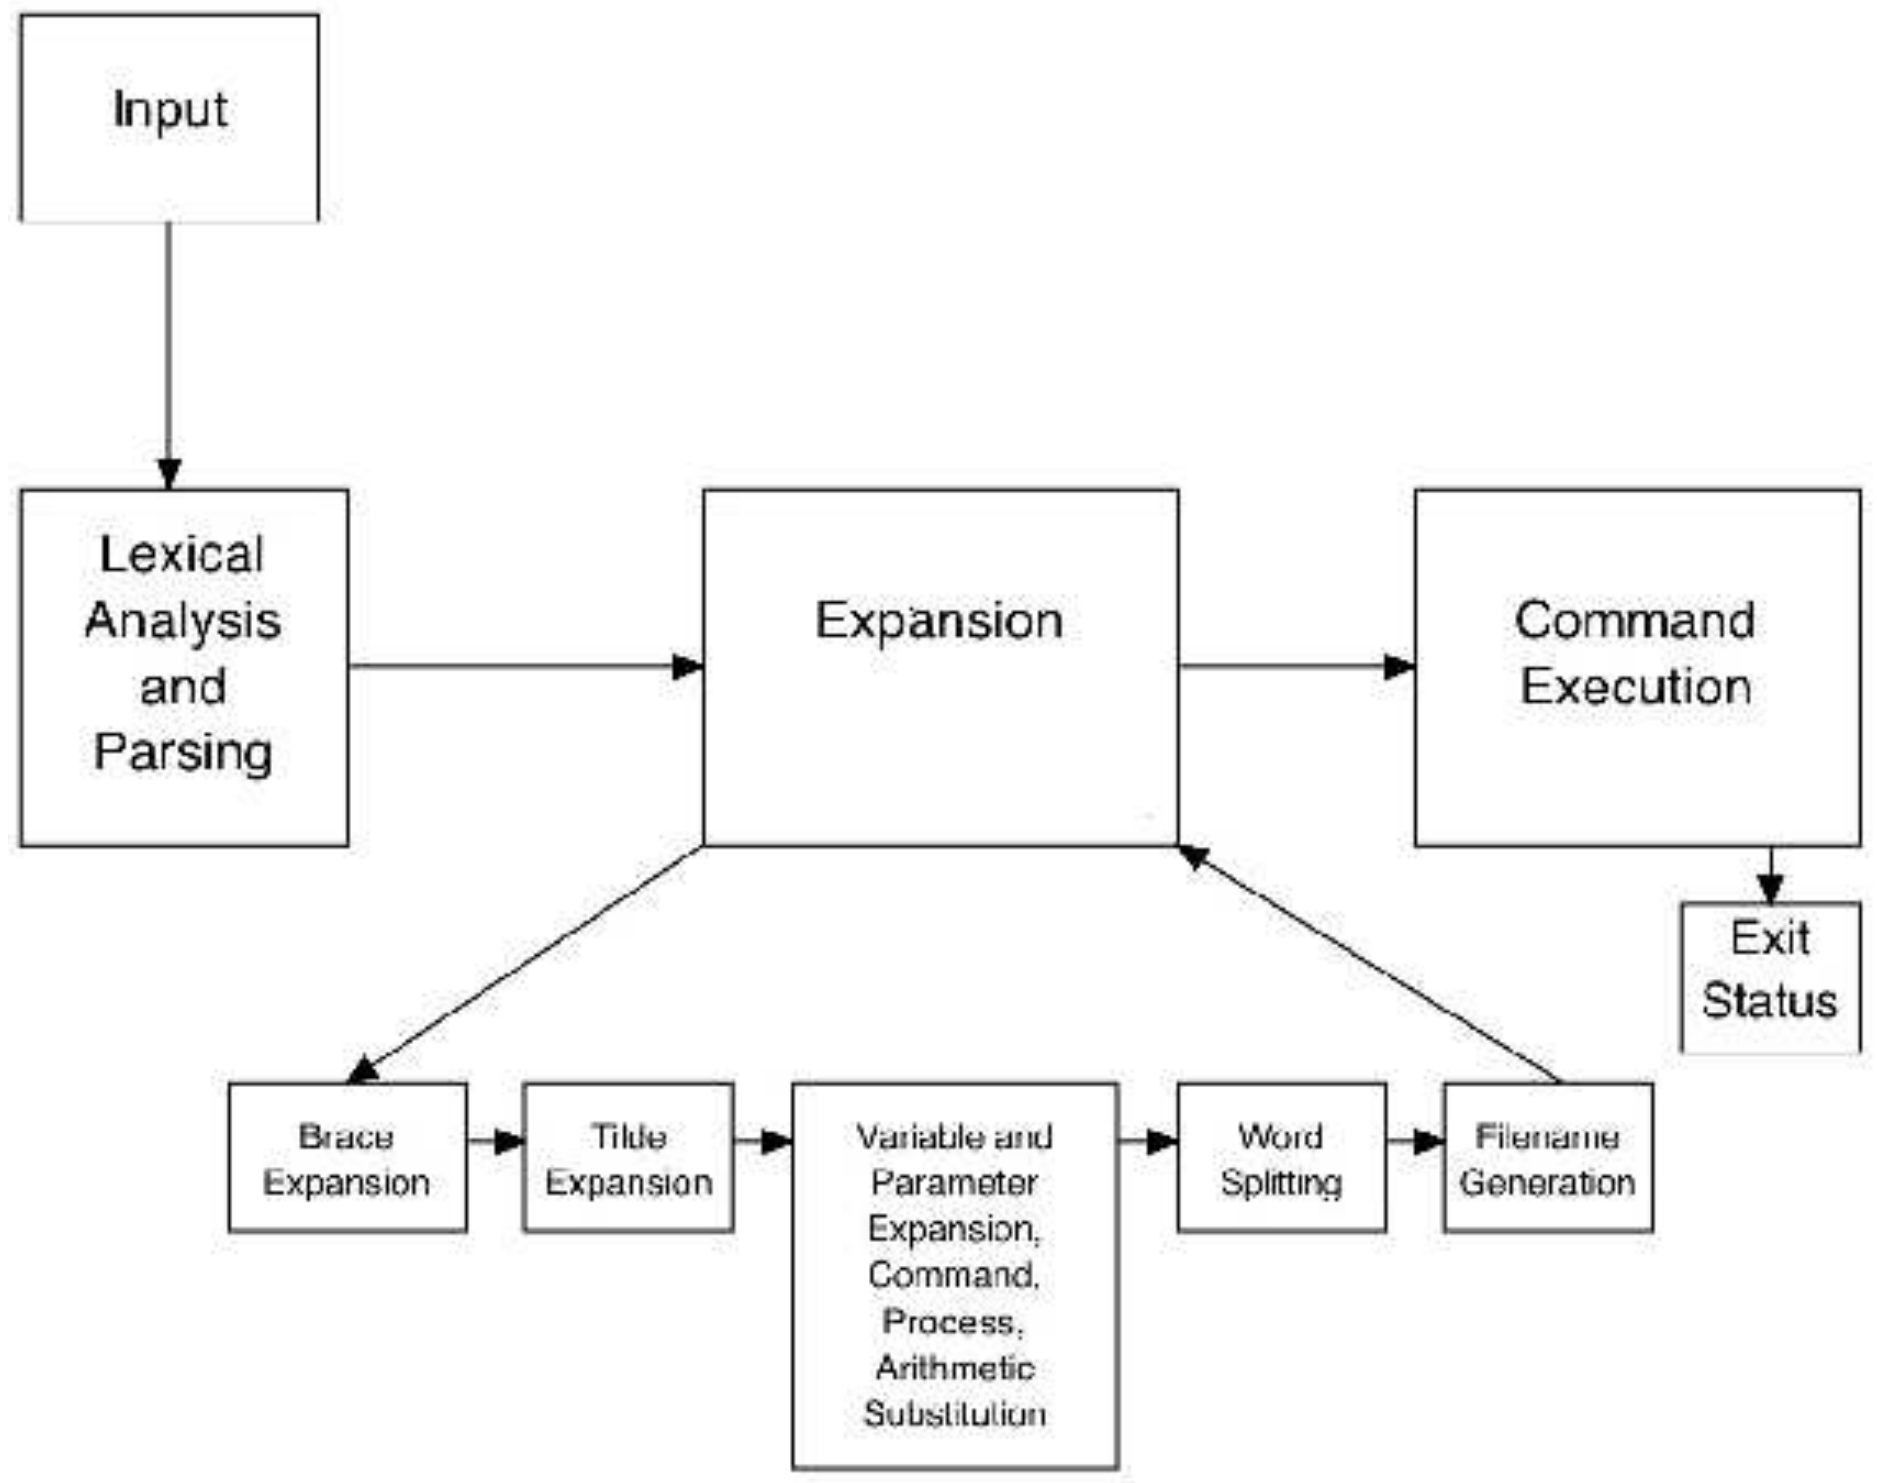
\includegraphics[width=0.7\textwidth]{bashArchitecture.png}
\end{center}

Диаграмма показывает поток данных между основными компонентами системы (в основном, Exit Status на самом деле компонентом системы не является, но я говорил, что неформальные диаграммы из квадратиков и стрелочек очень популярны и весьма полезны). Ввод (с консоли или из файла) поступает на вход лексическому и синтаксическому анализатору, далее последовательность слов, полученная парсером, отдаётся expansion-у, который на самом деле представляет собой конвейер, последовательно применяющий преобразования к последовательности слов. Сначала выполняется подстановка фигурных скобок, затем тильды, затем доллара, затем разделение на слова (после парсера, такие дела), затем раскрытие шаблонов. Дальше то, что получилось, подаётся на вход исполнялке команды, которая отвечает за перенаправление ввода-вывода, пайпы, группы процессов и т.д., в итоге получается результат выполнения команды в виде кода возврата.

Всё общение между компонентами выполняется с помощью структуры WORD\_DESC и различных контейнеров, содержащих эти структуры. Вот определение этой структуры:

\begin{minted}{c}
typedef struct word_desc {
    char *word; /* Zero terminated string. */
    int flags; /* Flags associated with this word. */
} WORD_DESC;
\end{minted}

А вот так, например, представляются аргументы команды:

\begin{minted}{c}
typedef struct word_list {
    struct word_list *next;
    WORD_DESC *word;
} WORD_LIST;
\end{minted}

\subsection{Ввод с консоли}

За ввод с консоли отвечает библиотека Readline, которая отвечает за редактирование командной строки и за хранение истории команд. Она устроена как цикл ``считать символ с клавиатуры - найти команду, ему соответствующую - исполнить её - показать результаты''. Символ считывается как 8-битный символ (в те времена, когда это писалось, юникода ещё не было) и используется как индекс в ``таблице диспетчеризации''. В этой таблице может быть либо команда (например, ``перейти в начало строки''), либо другая такая же таблица (это для поддержки сочетаний из нескольких символов), либо команда ``вывести считанный символ''. Ещё есть макросы (которые просто вставляют во входной поток символы). Все выводимые символы хранятся в буфере редактирования, а когда надо вывести результат на экран, Readline хитро рассчитывает минимальный набор команд управления курсором, который преобразует текущую отображаемую на экране строку в желаемую. Все внутренние данные хранятся в виде 8-битных символов, но Readline знает (теперь) про юникод и умеет его корректно отображать и корректно считать позиции для многобайтовых символов.

Readline может быть расширена добавлением произвольных функций в таблицу диспетчеризации, и Bash этим пользуется, добавляя более 30 своих команд (например, автодополнение).

\subsection{Синтаксический разбор}

Readline возвращает просто строку, введённую пользователем. Первое, что с ней делается --- лексический анализ, то есть, в случае с Bash-ем, разделение по словам и их идентификация. С последним дела обстоят довольно плохо, потому что смысл последовательности символов сильно зависит от контекста, так что лексер и парсер должны тесно общаться друг с другом, чтобы разбирать, например, вот такой ужас:

\begin{minted}{sh}
for for in for; do for=for; done; echo $for
\end{minted}

Эта команда, кстати, вполне корректна и выведет на экран ``for''.

Bash --- один из немногих шеллов, написаный на lex + bison, о чём, впрочем, автор несколько сожалеет, говоря, что ручная реализация рекурсивным спуском сильно упростила бы дело. Оригинальная грамматика шелла Борна, которую Bash пытается поддерживать, никому не известна, есть грамматика (контекстно-зависимая), стандартизованная POSIX, её-то и реализует Bash (так что грамматика Bash таки известна и документирована).

Интересно, что подстановка alias-ов выполняется лексером. Правда, для этого парсер сообщает ему, разрешена ли в данный момент подстановка. Лексер же отвечает за кавычки и бэкслеш.

Дополнительные проблемы создаёт подстановка результата выполнения команды и программируемое автодополнение, где тоже могут выполняться произвольные команды прямо в процессе разбора другой команды. Для поддержки таких вещей парсер умеет сохранять своё состояние и корректно восстанавливать его после разбора и исполнения ``подкоманды''.

Результат работы парсера --- одна команда (которая в случае сложных команд типа for может содержать подкоманды), которая передаётся модулю, отвечающему за подстановки.

\subsection{Подстановки}

Подстановки (expansions) работают на уровне слов и могут порождать новые слова и списки слов. Они могут быть довольно сложными, например,

\begin{minted}{sh}
${parameter:-word}
\end{minted}

раскрывается в \textit{parameter}, если он установлен, и в \textit{word}, если нет. А

\begin{minted}{sh}
pre{one,two,three}post
\end{minted}

раскрывается в 

\begin{minted}{sh}
preonepost pretwopost prethreepost
\end{minted}

Ещё бывает подстановка тильды и арифметическая подстановка. Все они выполняются по порядку, то есть подстановщики организованы во что-то вроде конвейера.

Результат подстановки снова разбивается на слова (при этом это делает код, видимо, отличный от лексера). После разбиения происходит замена шаблонов --- каждое слово интерпретируется как потенциальный шаблон и пытается сопоставиться с файлом в файловой системе.

\subsection{Исполнение команд}

Команды бывают встроенными (которые модифицируют состояние самого шелла, например, cd) и внешними, которые сами отдельные программы (например, cat). Ещё бывают сложные команды --- if, for и т.д.

Каждая команда позволяет перенаправлять свой ввод и вывод (да, даже в for можно направить входной поток из пайпа). Самое сложное в реализации перенаправления --- это следить за тем, когда его нужно отменить. Встроенные и внешние команды работают с точки зрения пользователя одинаково, поэтому наивная реализация перенаправления вывода встроенной команды перенаправила бы вывод всего шелла. При этом Bash ещё и следит за файловыми дескрипторами, которые участвуют в редиректе, создавая новые или используя старые при необходимости.

Встроенные команды реализованы как сишные функции, принимающие список слов как аргументы, и работают как ``обычные'' команды, только без запуска отдельного процесса. Единственная тонкость в том, что некоторые команды принимают как аргумент присваивания (например, export), они обрабатывают присваивание по-особому (для этого используются флаги в WORD\_DESC). Обычные присваивания (которые не в export или declare) реализованы на самом деле тоже как команды, но парсятся и обрабатываются немного по-особому. Если присваивание стоит перед обычной командой, то оно передаётся команде и действует до её завершения, если присваивание одно на строке, оно действует на весь шелл. 

Внешние команды перед запуском ищутся в файловой системе, при этом шелл смотрит на PATH. Но если в имени команды есть слеши, то не  ищет, а исполняет как есть. При этом единожды найдённая команда запоминается в хеш-таблице и дальше сначала ищется в ней (перехитрить Bash вроде не получится, если он по запомненному пути не нашёл, то пойдёт искать в PATH-е). Если команда не нашлась, Bash вызывает функцию, которую можно переопределить, и многие дистрибутивы это делают, предлагая поставить нужный пакет с командой.

Ещё есть некоторые хитрости с управлением процессами, в которых исполняются команды. Есть режим foreground, в котором шелл ждёт завершения процесса с командой, есть background, где шелл запускает команду и тут же читает следующую. При этом Bash умеет переводить команду из одного режима в другой, для чего там есть понятие ``Job'', как группа процессов, исполняющая команду. Например, пайпы собирают несколько процессов в один Job, который может быть отправлен в фон или в foreground целиком.

\subsection{Lessons learned}

Вот кратко вещи, на которые разработчик Bash Chet Ramey обратил внимание в ходе разработки.

\begin{itemize}
	\item Хорошие комментарии к коммитам со ссылками на багрепорты с шагами воспроизведения сильно облегчают жизнь.
	\item Хороший набор тестов --- тоже, Bash имеет тысячи тестов, покрывающие практически всю неинтерактивную функциональность.
	\item Сильно помогли стандарты, как внешние на функциональность шелла, так и внутренние на код.
	\item Хорошая пользовательская документация важна.
	\item Переиспользование сильно экономит время.
\end{itemize}

\subsection{Как обстоят дела на самом деле}

Товарищи из университета Южной Калифорнии исследовали ``настоящую'' архитектуру Bash с целью получить ``базовую'' архитектуру, по которой можно было бы оценивать эффективность различных инструментов автоматического восстановления архитектуры. Один аспирант 80 часов копался в исходниках, после чего отправил результаты автору и тот ещё высказал свои соображения. В итоге получилась вот такая структура системы:

\begin{center}
	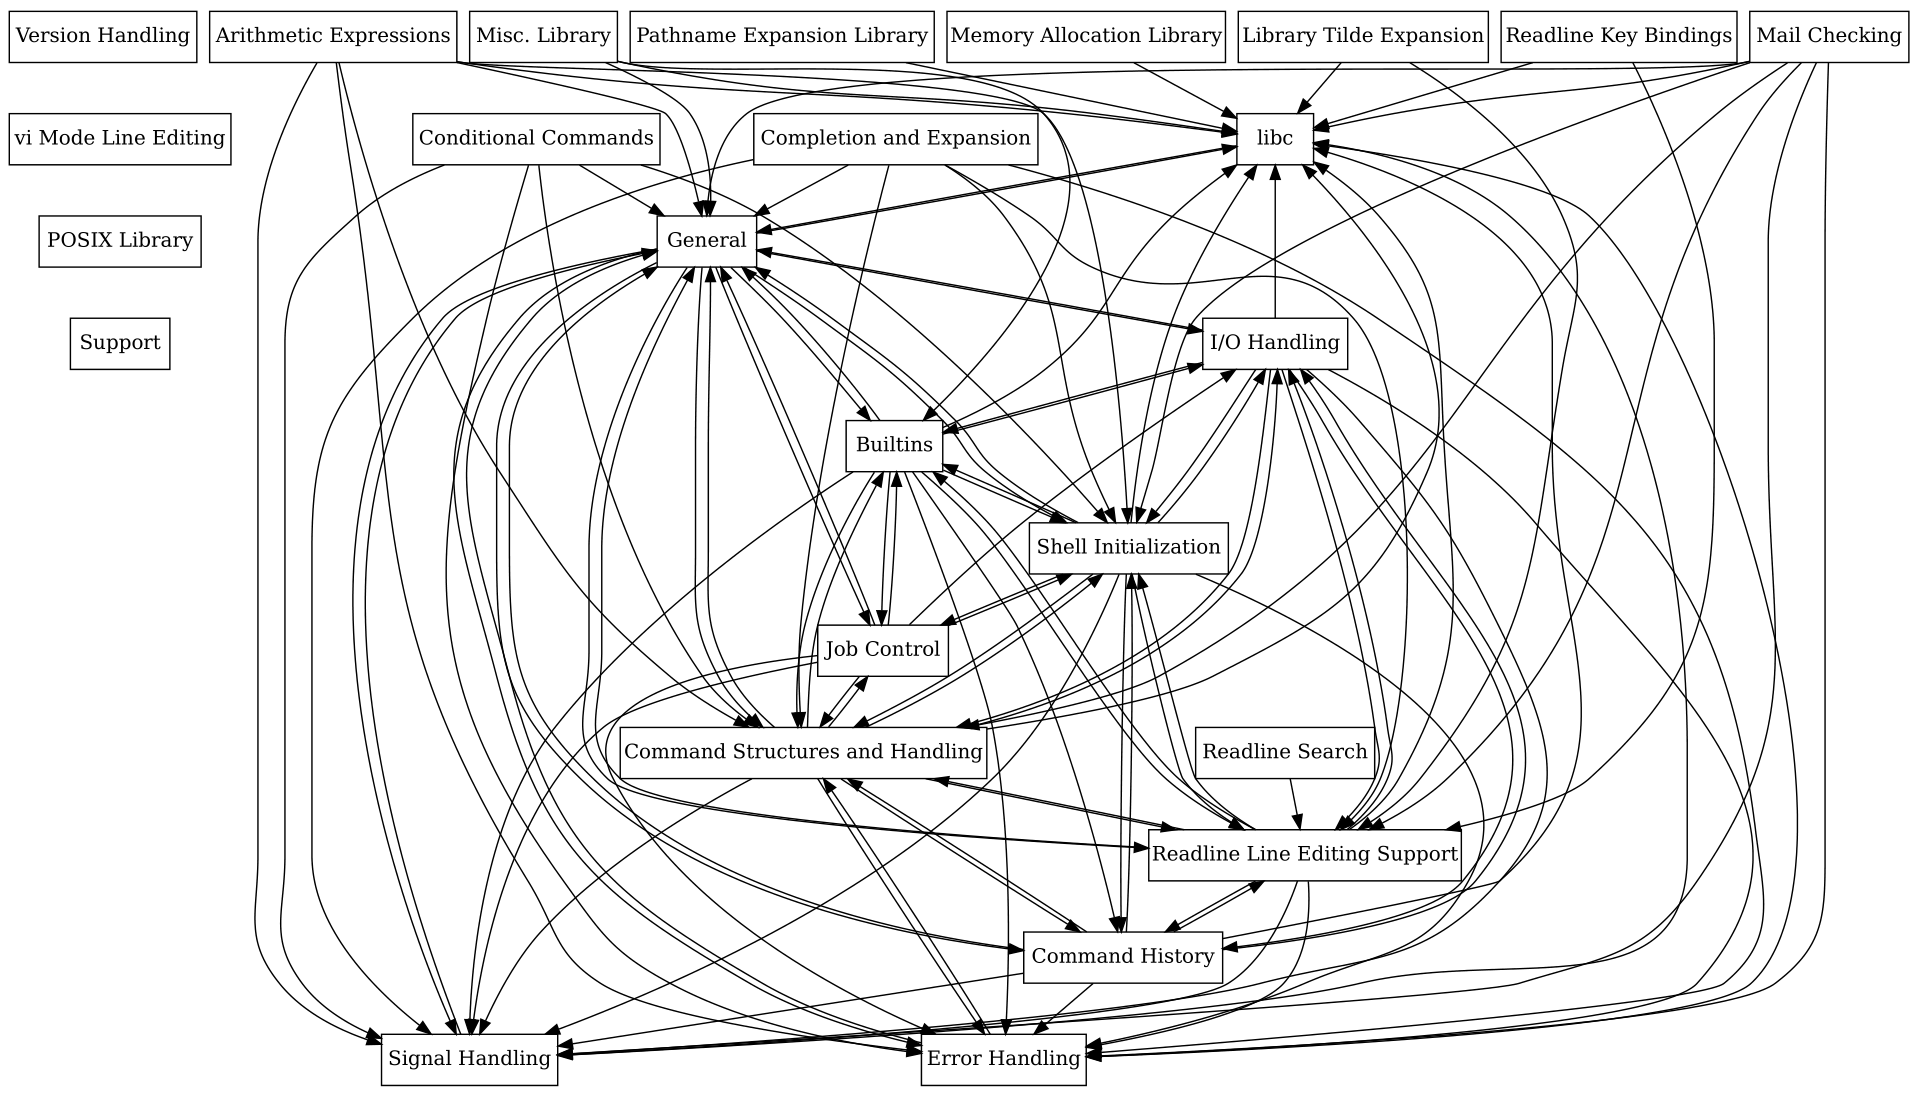
\includegraphics[width=\textwidth]{bashRealArchitecture.png}
\end{center}

Видно, что зависимостей в коде больше, чем на картинке с концептуальной архитектурой и поток данных на структурной диаграмме совершенно неочевиден. Но некоторые схожести всё-таки есть, например, ввод-вывод реально выделяются в отдельный кластер компонентов.

Bash имеет размер порядка 70К строк кода, около 200 отдельных файлов. В ходе восстановления архитектуры было выделено 25 компонентов, из которых 16 относятся к ядру функциональности системы, 9 --- вспомогательные. Выяснилось, что структура папок практически не соответствует компонентам, только два компонента имеют свои отдельные папки в исходниках.

Вот автоматически восстановленная по исходникам архитектура системы, с компонентами и зависимостями:

\begin{center}
	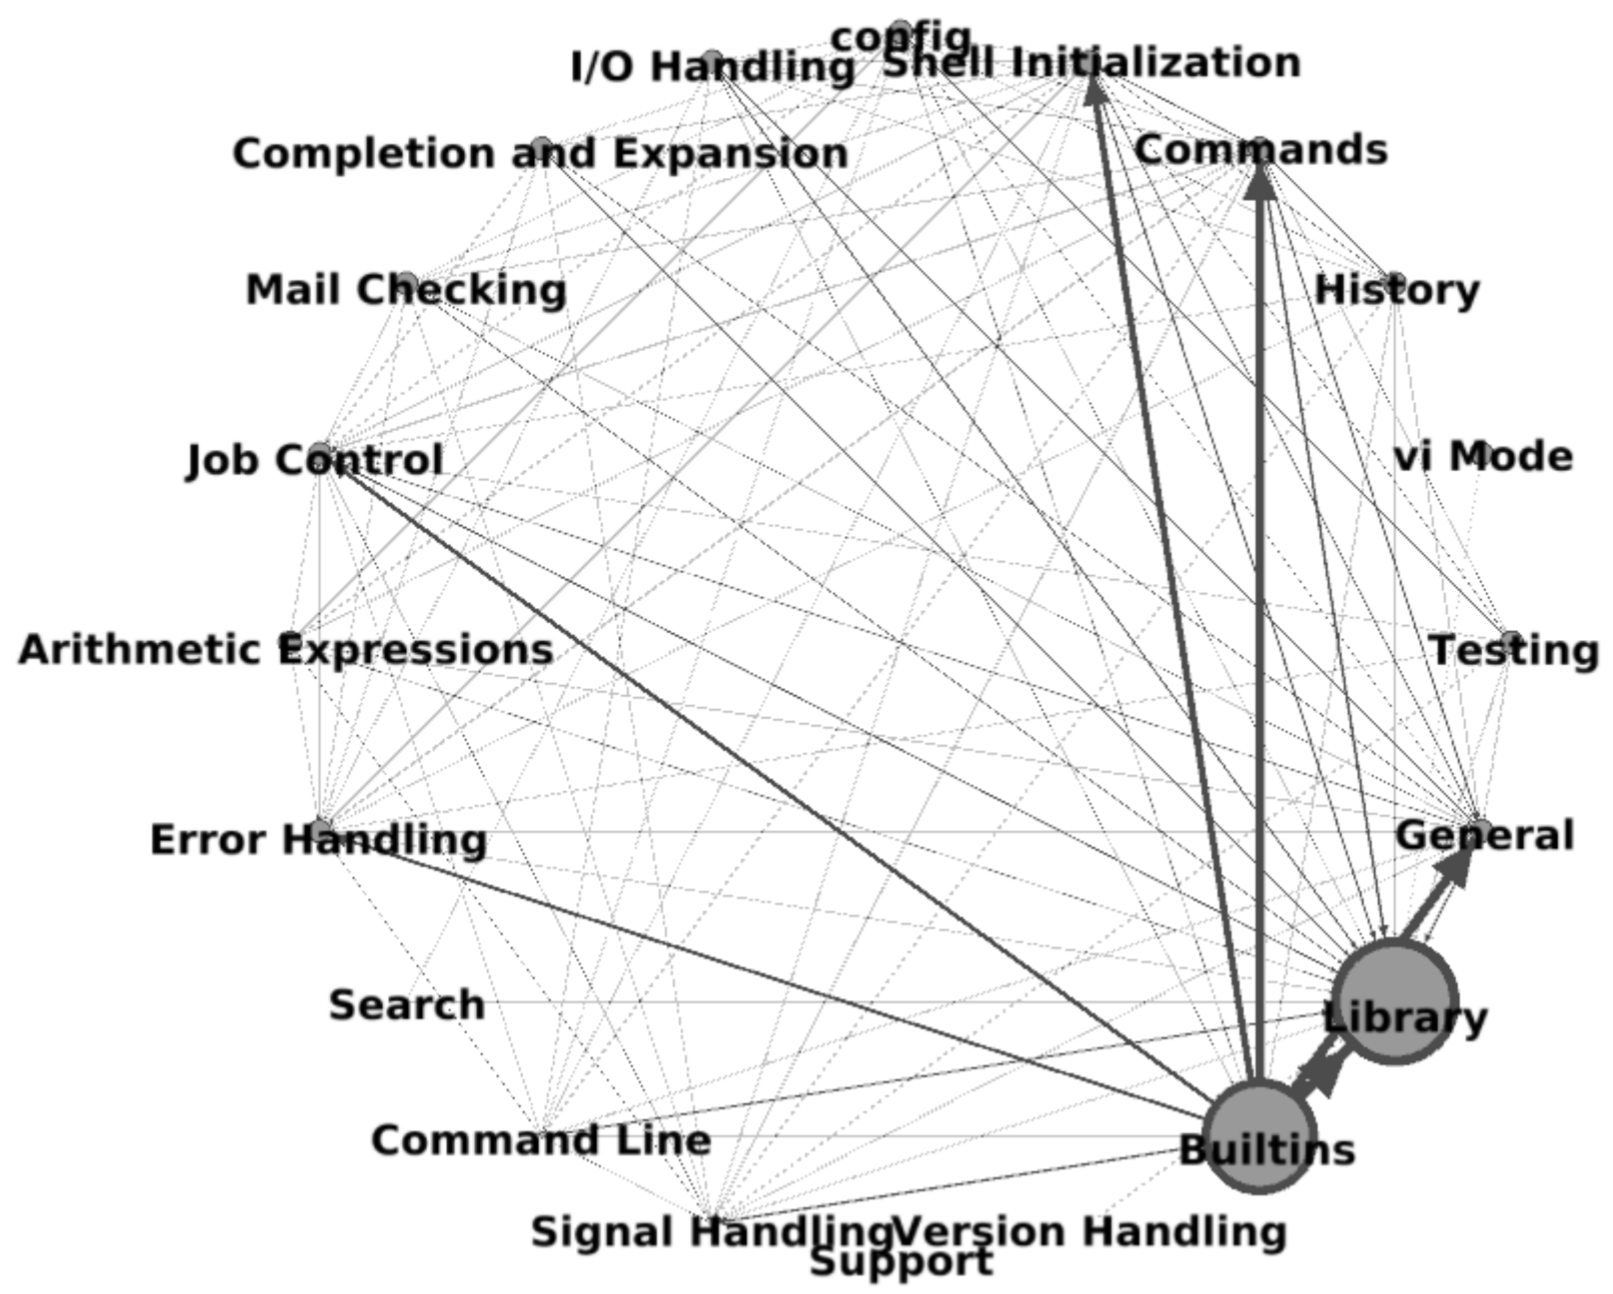
\includegraphics[width=0.7\textwidth]{bashAutomaticRecoveryArchitecture.png}
\end{center}

Сравните с исходной концептуальной архитектурой:

\begin{center}
	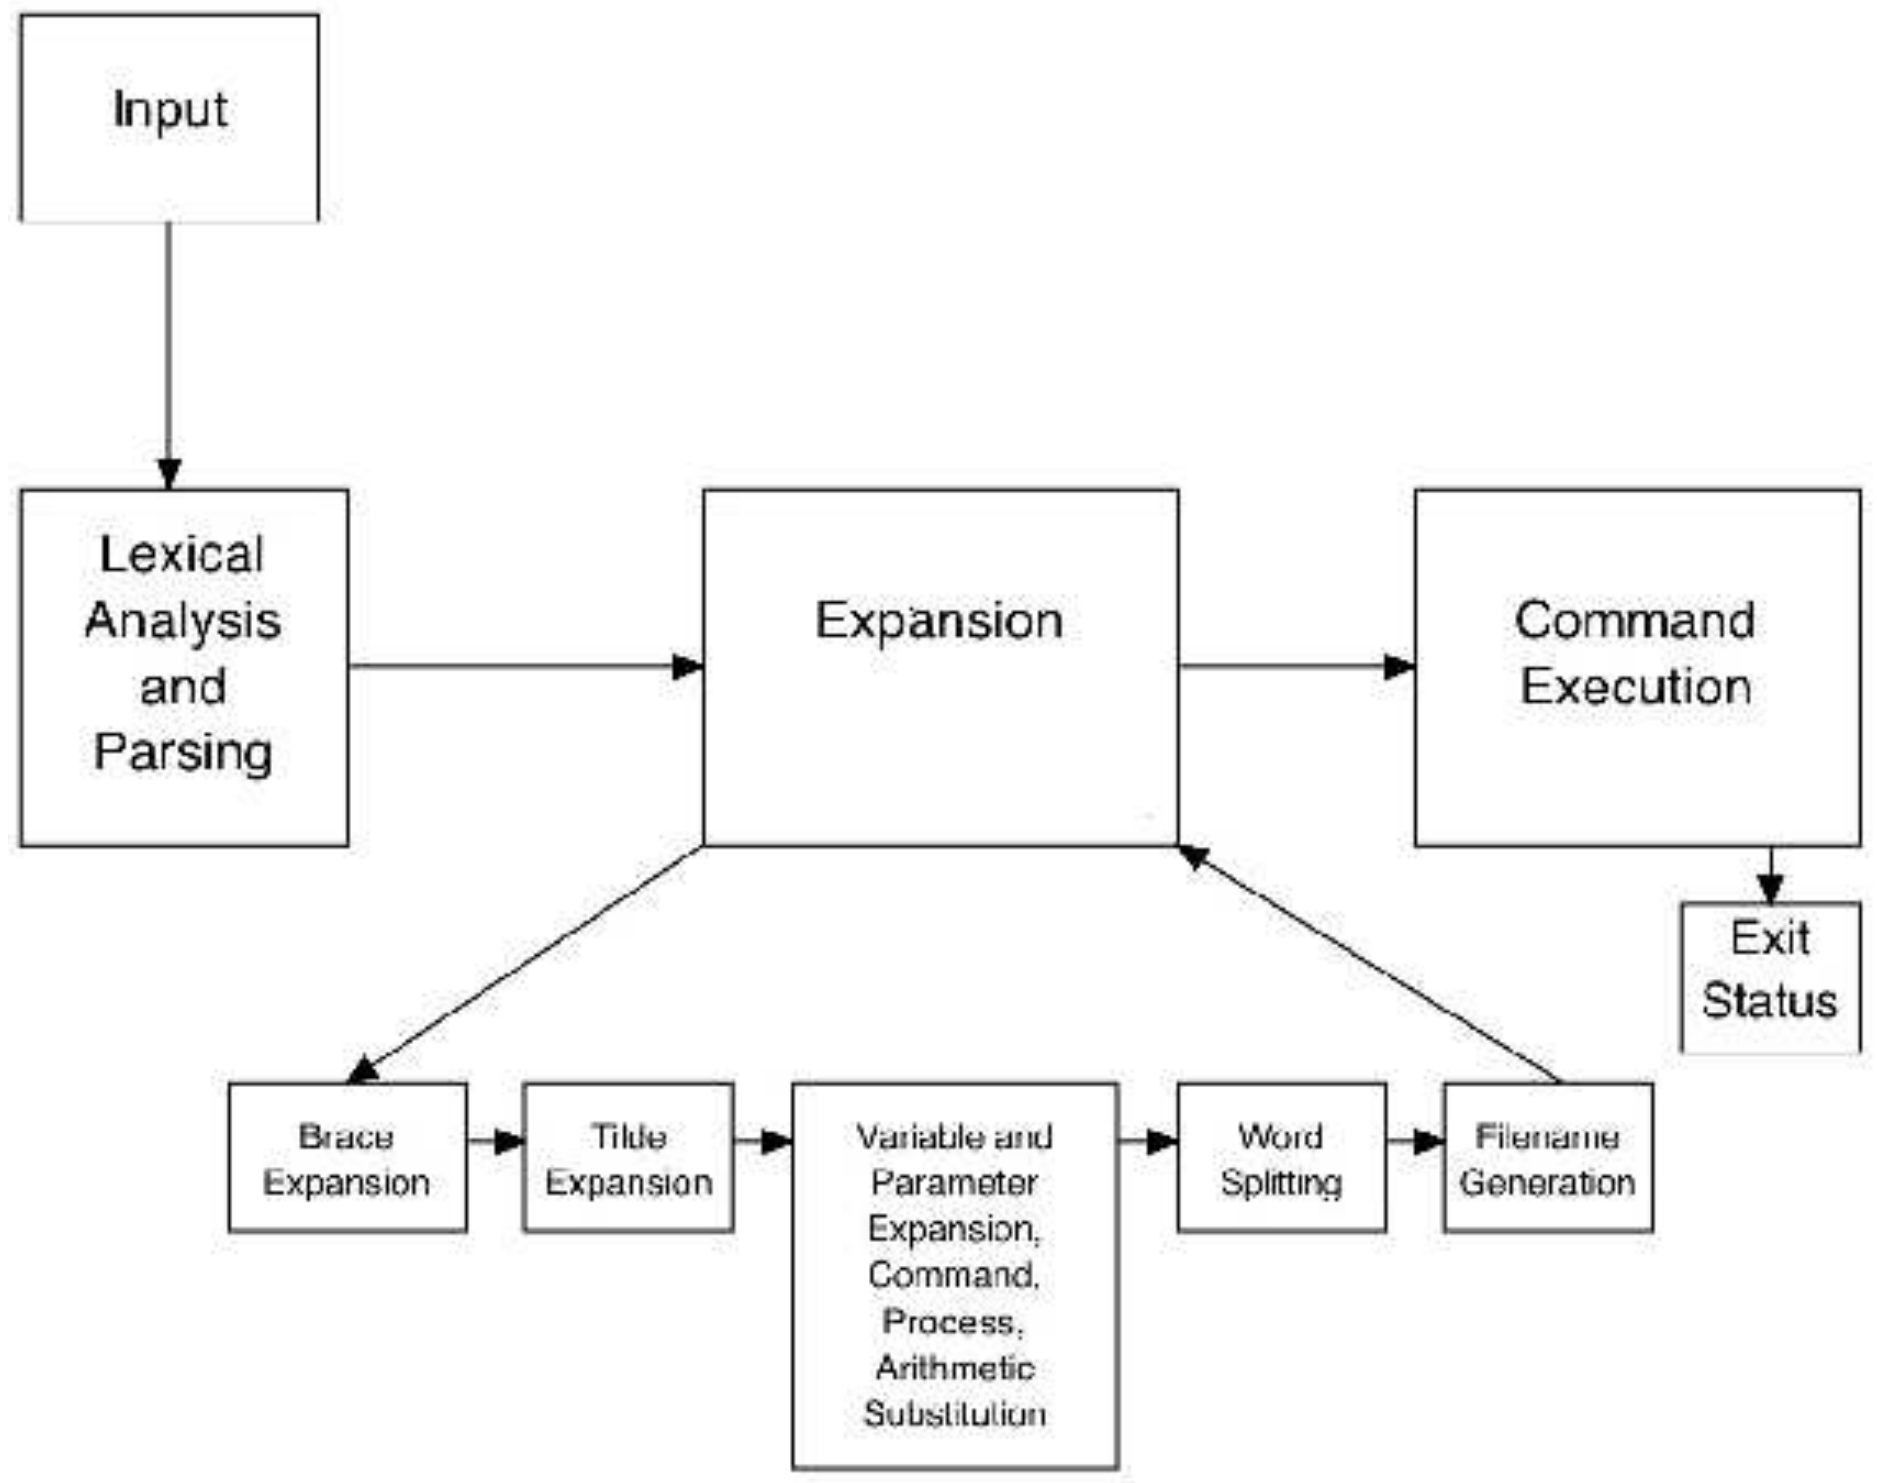
\includegraphics[width=0.6\textwidth]{bashArchitecture.png}
\end{center}

Это должно подвести к важной мысли касательно архитектур реальных приложений --- есть архитектура как она проектировалась (prescriptive architecture), есть архитектура как она реализована в коде приложения (descriptive architecture), и в ходе эволюции приложения эти архитектуры становятся всё больше и больше непохожими друг на друга. Эти расходждения связаны с понятиями ``architectural drift'' (привнесение в архитектуру вещей, которых в исходной архитектуре на было, без нарушения принципов исходной архитектуры) и ``architectural erosion'' (привнесение в реализацию нарушений принципов исходной архитектуры). Для долгоживущих систем архитектурная эрозия становится довольно критичным фактором, приводящим к тому, что исходное разбиение на компоненты перестаёт быть валидным вообще. Bash в этом плане довольно показателен, поскольку ему много лет. Вот увеличенный вид компоненты управления Job-ами:

\begin{center}
	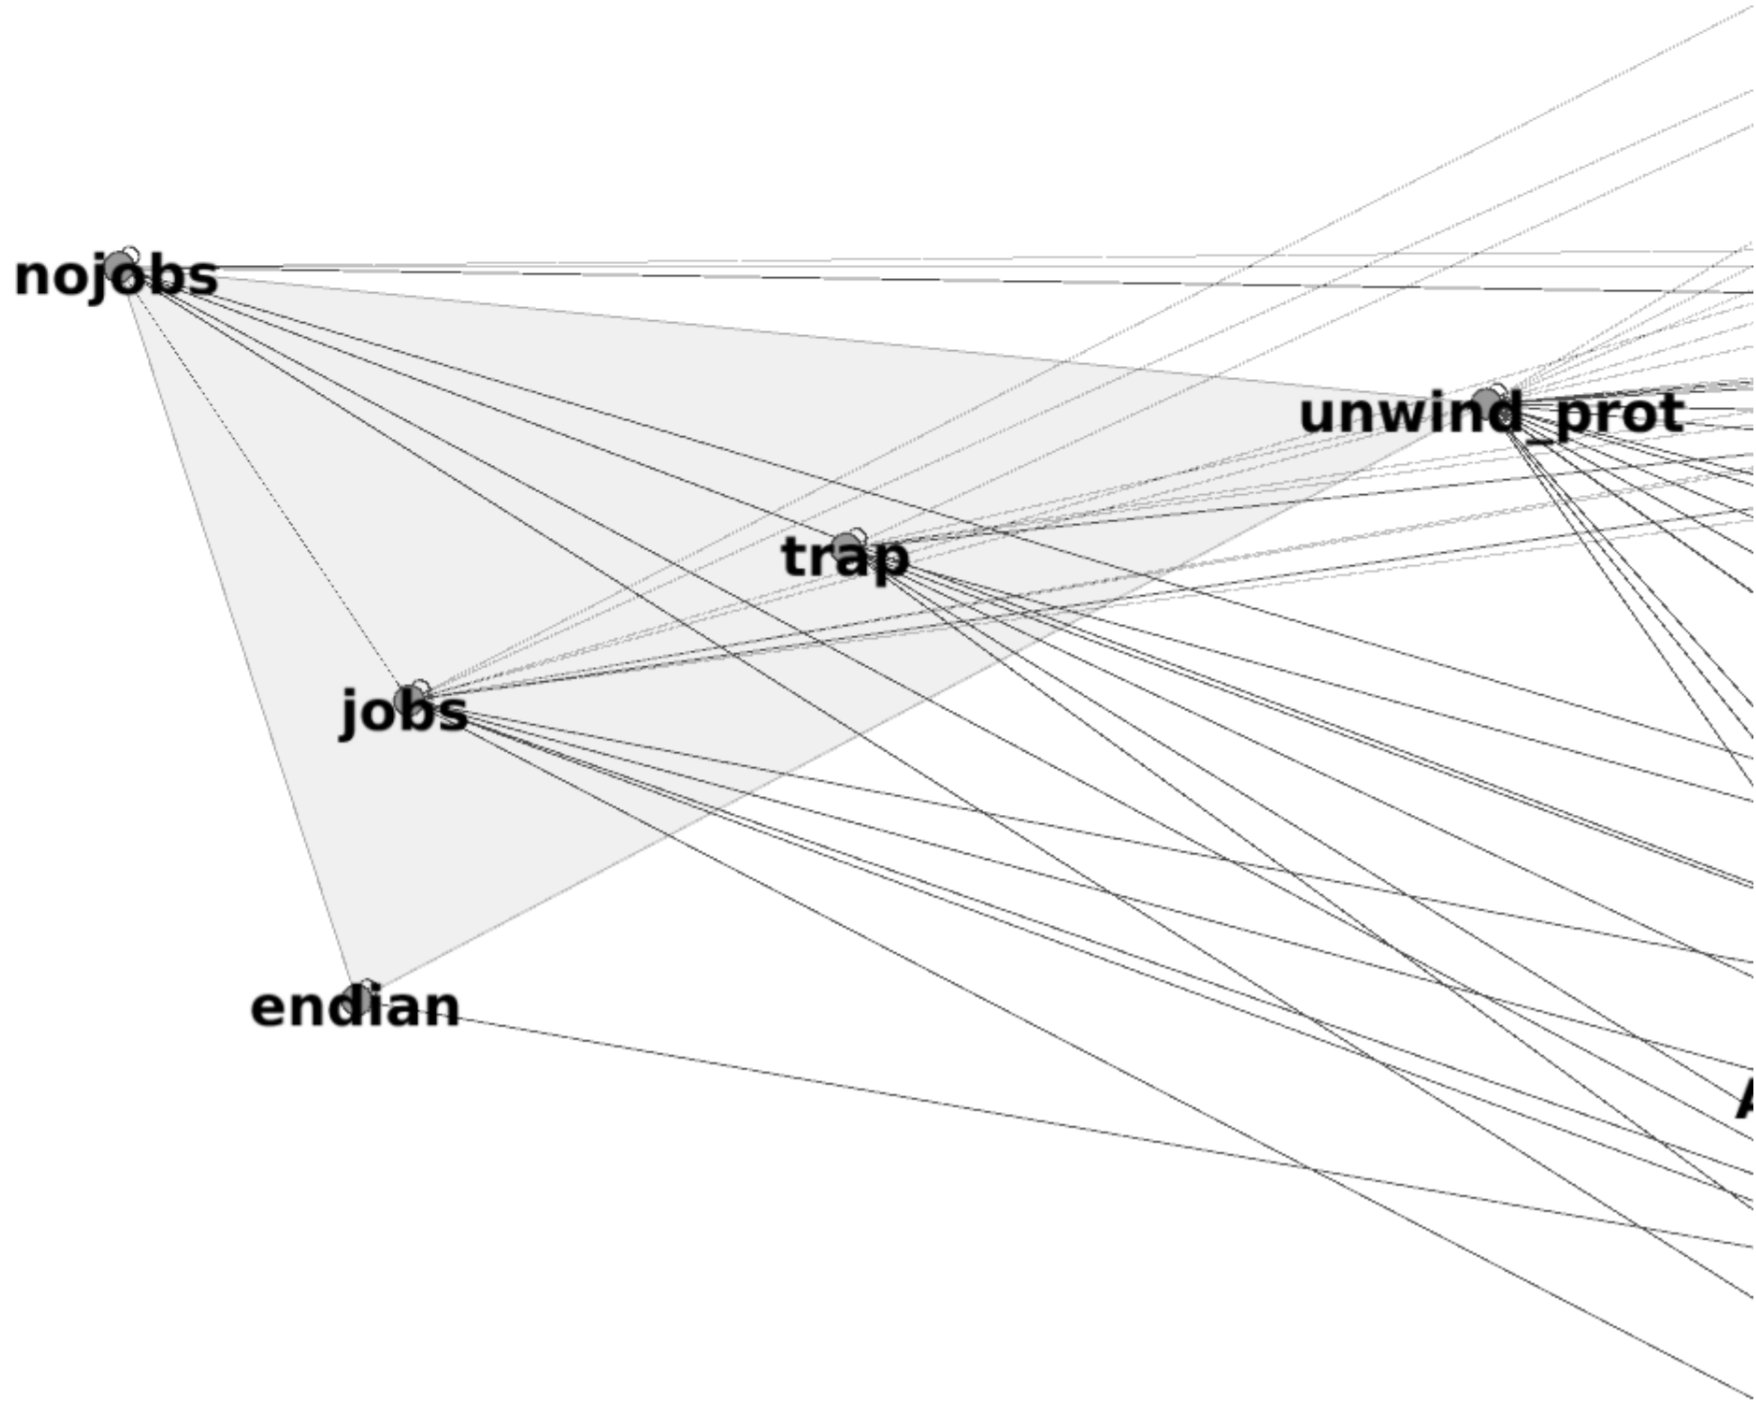
\includegraphics[width=0.6\textwidth]{bashJobControl.png}
\end{center}

Как видим, каждая сущность с этой компоненте больше связана с внешними сущностями, чем с сущностями внутри компоненты, то есть coupling очень высок, а cohesion, судя по всему, очень низок. С командами дела обстоят ещё хуже:

\begin{center}
	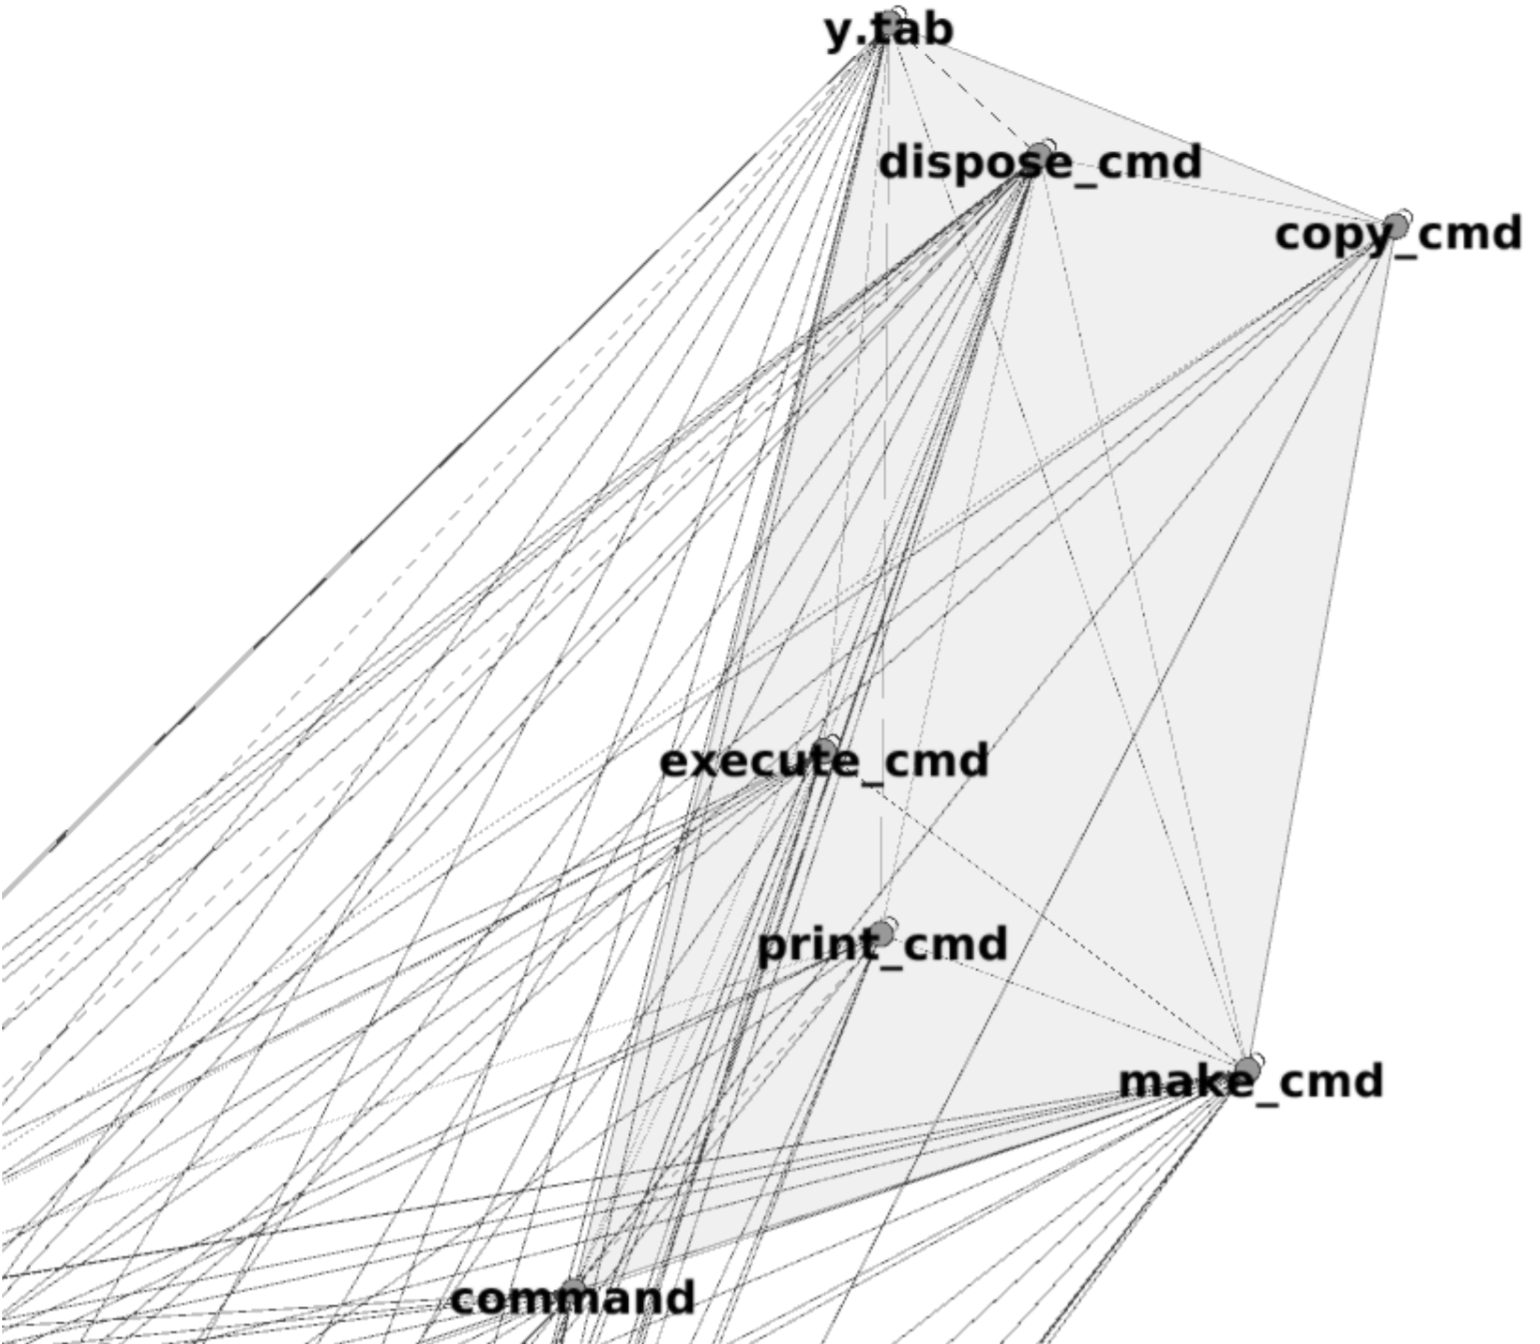
\includegraphics[width=0.6\textwidth]{bashCommands.png}
\end{center}

Собственно, поэтому важна архитектурная документация и нелишне наличие архитектора, который следил бы за тем, чтобы код и документация не очень расходились. Иначе приложение быстро превратится в гигантский ком кода, где всё зависит от всего и ломается при любом изменении.

\section{Grep}

Следующая домашняя задача --- реализовать в рамках существующего CLI (ну, у большинства --- пока потенциально существующего) команду grep, которая бы искала подстроки в файле или входном потоке. Весь синтаксис grep-а поддерживать не надо, надо уметь принимать регулярные выражения (так, как они реализованы в вашем любимом языке программирования, писать свой парсер регэкспов не нужно) и поддерживать ключи:

\begin{itemize}
	\item \textit{-i} --- нечувствительность к регистру;
	\item \textit{-w}  --- поиск только слов целиком;
	\item \textit{-A n} --- распечатать n строк после строки с совпадением.
\end{itemize}

Вот некоторое количество примеров вызова того, что должно получиться:
\begin{minted}{bash}
> grep plugin build.gradle
    apply plugin: 'java'
    apply plugin: 'idea'
> cat build.gradle | grep plugin
    apply plugin: 'java'
    apply plugin: 'idea'
> grep -A 2 plugin build.gradle
    apply plugin: 'java'
    apply plugin: 'idea'
    group = 'ru.example'
    version = '1.0'
\end{minted}

С архитектурной точки зрения эта задача интересна тем, что писать разбор аргументов командной строки вручную --- это дело муторное и, кажется, широко распространённое (существуют тысячи консольных утилит, они ведь должны как-то парсить свои аргументы). Поэтому, как обычно, перед тем, как кидаться что-то кодить, надо поискать уже готовые опенсорсные решения. Собственно, это одна из самых важных задач архитектора --- во-первых, чувствовать, где можно применить третьесторонние компоненты, а где проще реализовать самим, во-вторых, уметь совершать обоснованный выбор третьесторонней компоненты среди аналогов, в-третьих, знать кучу всего, чтобы иметь возможность сказать <<ага, а вот есть такая штука, она делает то, что нам надо! (и у неё наверняка есть аналоги, потому что я слышал о ней уже три года назад, она наверняка протухла)>>.

Каких-то неочевидных практик поиска третьесторонних компонент, наверное, не существует, вот немножко очевидных рекомендаций, на всякий случай.
\begin{itemize}
	\item Миллион леммингов не может ошибаться, поэтому у хорошей либы наверняка много пользователей (правда, тут следует брать поправку на год появления), быстрое гугление покажет, насколько активно сообщество на GitHub, StackOverflow и подобных местах.
	\item Даже если компонента очень хороша, маленькое сообщество приведёт к проблемам --- негде будет найти предыдущий опыт, труднее будет получить совет, если что-то пойдёт не так.
	\item Если есть несколько фаворитов, имеет смысл потратить время на то, чтобы поковыряться с ними со всеми и выбрать то, что больше подходит или даже просто больше понравилось. Пробовать прежде всего стоит то, что кажется сложным, потому что часто бывает, что что-то простое делается просто, а сложное --- вообще никак, и придётся отказаться от выбранной компоненты посреди процесса интеграции. 
	\item Обращайте внимание на лицензию. Даже лицензия типа GPLv3 может быть showstopper-ом для использования идеальной во всех остальных отношениях компоненты. Ни один нормальный архитектор не интегрирует в свою систему компоненту, которая хотя бы потенциально может иметь проблемы с авторскими правами.
	\begin{itemize}
		\item Поэтому если вы всё ещё выкладываете код на GitHub без явного указания лицензии, подумайте, достаточно ли добродетельный вы человек. Код без лицензии по большинству законов использовать может только автор, даже если он лежит в открытом доступе.
	\end{itemize}
\end{itemize}

Хочется, чтобы на этом простом примере вы попробовали сделать обоснованный выбор библиотеки разбора параметров командной строки. Выбор может быть не очевиден, но сами по себе такие библиотеки не очень сложные, так что тут реально хорошо подходит тактика <<попробовать все и выбрать то, что пришлось по душе больше>>. Тем не менее, мы <<играем во взрослые проекты>>, поэтому хочется в домашнем задании текстовый документ с описанием того, какие библиотеки были рассмотрены, их достоинства и недостатки и почему была выбрана именно та библиотека, которую вы в итоге выберите. Аргумент <<Я всю жизнь ей пользовался>> считается в данном случае невалидным.

\end{document}
